%% LyX 2.0.6 created this file.  For more info, see http://www.lyx.org/.
%% Do not edit unless you really know what you are doing.
\RequirePackage{fix-cm}
\documentclass[english]{article}
\usepackage[LGR,T1]{fontenc}
\usepackage[latin9]{inputenc}
\setlength{\parskip}{\medskipamount}
\setlength{\parindent}{0pt}
\usepackage{amsmath}
\usepackage{amssymb}
\usepackage{fixltx2e}
\usepackage{graphicx}

\makeatletter

%%%%%%%%%%%%%%%%%%%%%%%%%%%%%% LyX specific LaTeX commands.
\DeclareRobustCommand{\greektext}{%
  \fontencoding{LGR}\selectfont\def\encodingdefault{LGR}}
\DeclareRobustCommand{\textgreek}[1]{\leavevmode{\greektext #1}}
\DeclareFontEncoding{LGR}{}{}
\DeclareTextSymbol{\~}{LGR}{126}

%%%%%%%%%%%%%%%%%%%%%%%%%%%%%% Textclass specific LaTeX commands.
\numberwithin{equation}{section}
\numberwithin{figure}{section}
\numberwithin{table}{section}

\makeatother

\usepackage{babel}
\begin{document}

\title{Automated Routing in Pedestrian Dynamics}


\author{Arne Graf}


\date{2015-09-01}

\maketitle

\newpage

\section*{Abstract}
In dieser Arbeit wird genommen: Model von Felix, Bodenfeld von Madrid, Code adaptiert von Leonardo Andr�s Zepeda N��ez. 
Es wird ein Testmodel beschrieben, welches den Einflu� des Madrid-Bodenfeldes untersucht.
Historie: Dietrich's Model in Jupedsim; Bodenfeld warf Frage auf: Welche Diskretisierung (rectGrid, triangulated, how to deal with wall-surfaces), Probleme durch non-smooth Bodenfeld (?); -> Beschluss: Bodenfeld so gestalten, dass es gute Eigenschaften bei der Fu�g�ngersimulation verspricht. 
Dieses dann untersuchen und qualifizieren. Durch die Betreuung von M.C. floss die Erfahrung zahlreicher Modelle ein und bei der Modelfindung ein geeignetes Testmodel neu beschrieben.

In this thesis, the effect of an alternate floor-field was analyzed, by using it in a newly composed test-model for pedestrian dynamics. In the simulation
of pedestrian (crowd) movement, the routing of agents\footnote{An agent is the representation of a pedestrian in the simulation. Depending on the used
model, an agent incorporates some kind of artificial intelligence or basic agent-attributes only (like size, speed attributes, etc.). In the latter case the model takes over
the task of navigating agents.} is an integral part. Routing can be seen as the composition of two aspects: the global pathfinding through a geometry
and the avoidance of static or dynamic obstacles\footnote{collision detection} (like walls or other agents) in a local\footnote{local in time and/or in space} situation.

The history of pedestrian simulation shows various models with different answers to the
question of navigation. Many of which make use of manually added elements\footnote{like some sort of domain-decomposition, e.g. through helplines} to solve the global pathfinding, which enable the user to simulate crowd movement in that very geometry. Other models use an automated algorithm, that will supply a navigation direction calculated from the agent's current position, the goal (area) and the geometry data.
The model described by F. Dietrich is one of the later. It uses the solution of the Eikonal Equation (see chapter \ref{eikonalequation}), which describes a 2-D wave-propagation. The wave starts in the target region and propagates through the geometry. To navigate agents, they are directed in the opposing direction to the gradient of said
solution of the Eikonal Equation. It is to be noted, that the solution of the Eikonal Equation can be calculated beforehand and does not contribute to the runtime of any given simulation scenario.
The Routing using the plain floor-field will yield non-smooth pathways as described later. This could pose a problem for some models. Dietrich shows the existance and uniqueness of his problem-formulation by using the theorem of Picard-Lindel�f. To apply this theorem, the smoothness of the input-functions must be given. Dietrich solves that problem by the use of a mollifier, which basically takes anything and gives you a smooth approximation of the input.
In this thesis, a floor-field is described, which solves the issue (non-smoothness) as a welcome side-effect. The research-group in Madrid (add ref) is working on the safe navigation of robots through a geometry. Robots are not to follow paths, which cut corners (which come close to any obstacles). A so-called distance-map is created and used as we see later. The welcome side-effect is smooth pathways by the the avoidance of walls and corners. The researchers take that approach even further, by reducing any geometry into a graph of edges and knots and thus having the domain in which the 2-D wave propagates reduced dramatically. Their intent is to calculate the floor-field in real-time using it for the reduced view-field of the robot's sensors.
Our interest in this trick (wording..) is different. We welcome the smoothness of the resulting pathways and take special interest in the behavior of agents close to obstacles. The floor-field itself shows pathways, which show a repulsive character in the vector-field. This phenomenon enables us to formulate a new model, one that uses an altered floor-field. Thanks to the rich experience of Chraibi in creation and testing of pedestrian dynamics models, we followed his intuition to use that altered floor-field in a new model. The results seen in the simulations show remarkably good behavior. The model is easy to use, fast and shows superior characteristics in routing through complex geometries. The extent to which we alter the floor-field is subject to our analysis.

\newpage
\tableofcontents 
\newpage

\section{Pedestrian Dynamics: Introduction}
<< big picture: micor-/macroscopic models, cell automata/ODE-based, 
take a closer look in next chapter >>
Pedestrian Dynamics defines a field of research trying to understand the underlying concepts (kinematics or kinetics? check..) and mechanics of pedestrian crowd movement. Understanding how crowd behavior will react in different situations (geometries), will lead to the ability to design our environment to best fit the needs to safely conduct large events, design buildings (traffic infrasturcture) to safely move large amounts of people through train stations even during rush hour.

\section{ODE based Model}

<< Explain different types (social force (2nd order), velocity based (1st order)) >>

<< velocity based have a sub-group using floor-fields (Dietrich's) >>

<< yet another model? >>

\section{Modelling}

In the latter, a new model is described, 
\begin{itemize}
\item aiming for
the avoidance of faulty interaction of pedestrians and walls 
\item while
maintaining the positive characteristics of row-formation, stop-and-go
waves and such - like seen in pedestrian crowd behavior/experiments/reality. (split up into more sentences).
\end{itemize}
In many of the existing
models (using mathematical formulations in the continuous space/domain), agents
breach wall-surfaces and get stuck inside of walls.
%\footnote{This agent-behavior in simulations has not yet been observed in experiments. Participants asked to do so in advance refused cooperation. (just kidding)}
This undesired phenomenon 
shows the challenge in calibrating forces and parameters of existing models, so that agents show valid natural behavior while not getting
overlapping in extreme situations. Especially in situations of high crowd density, e.g. when facing bottlenecks, 
overlapping can occur.
The model or the data-post-processing needs to find a special treatment of such artifacts in the data. It leads 
to problems in counting, flow-calculation, simulation-stop-criterium and such.

There are three mechanics used in the model to avoid ``overlapping/clipping'' in the vicinity of walls (include a figure for each):
\begin{enumerate}
\item The routing of pedestrians makes use of the eikonal-equation, computed
with an inhomogeneous speed-function, $s(x)$, whose resulting floor-field\footnote{see chapter \textbf{Eikonal Equation, Safe Navigation using the Floor-field}} favors keeping
a distance to obstacles, walls and corners.
\item The angle between an agent's moving-direction and the wall-surface-perpendicular affects the moving
speed if and only if the agent's moving vector includes a component
geared towards the wall.
\item If an agent's distance to a wall drops below a fixed parameter, he is redirected to 
move parallel to the wall if and only if the agent's moving vector includes a component
geared towords the wall.
\end{enumerate}

In order to keep the model simple, repulsive wall forces as seen in
Social Force Models are omitted. An analogy to repulsive pedestrian
forces though is used to keep agents from colliding with each other.
The model differs from SFMs, as in SFMs, other agents repulsive forces are transformed into acceleration
vectors and from there into a velocity component, which is part of the agent's velocity.
In this model though, repulsive forces are not treated as Newton mechanics teaches us, but are only used to 
factor the repulsive pedestrian effect into a direction component. The magnitude on the other hand is effected by the
other agents only to a certain degree (as discussed below).

\vspace*{2cm}

\textbf{Definitions:}

\begin{tabular}{lllclll}
$ d \quad $ & : $\Omega $ & $ \ni \vec{x} $ & $ \longrightarrow $ & $ d(\vec{x}) $ & $\in \mathbb{R} \quad $ & $:=  \quad $ distance to the closest wall \\
$ P $ & : $\mathbb{R}^2 \times \Omega $ & $ \ni (\vec{v}, \vec{x}) $ & $ \longrightarrow $ & $ P(\vec{v}, \vec{x}) $ & $\in \mathbb{R}^2 \quad $ & $ := \quad  $ orth. proj. of $\vec{v}$ onto closest wall of $\vec{x}$ \\
$ v_{ff} \quad $ & : $\Omega $ & $ \ni \vec{x} $ & $ \longrightarrow $ & $ v_{ff}(\vec{x}) = \vec{v}_{ff} $ & $ \in \mathbb{R}^2 \quad $ & $:=  \quad $ floor-field at position $\vec{x}$ \\
$ g $ & : $\mathbb{R}^2 $ & $ \ni \vec{v} $ & $ \longrightarrow $ & $ g(\vec{v}) $ & $ \in \mathbb{S}^2 $ & $:= \quad $ proj. onto the unit-sphere in $\mathbb{R}^2$ \\
\end{tabular}

\vspace*{2cm}

\textbf{Variant Model:}
\begin{align*}
&\Delta\vec{x}_{n}&&= \Delta t\cdot\vec{v}_{n, res}\\
&\vec{v}_{n, res}&&= \left\{
	\begin{aligned}
	    &\left(1-\frac{1}{2}\left[(\hat{v}\cdot(-\nabla \hat{d}))+\vert(\hat{v}\cdot(-\nabla \hat{d}))\vert\right]\right)  & P(\vec{v}_{n}) \quad &: & d(\vec{x})&& < 0.1\\
		&\left(1-\frac{1}{2}\left[(\hat{v}\cdot(-\nabla \hat{d}))+\vert(\hat{v}\cdot(-\nabla \hat{d}))\vert\right]\right)  & \vec{v}_{n} \quad  &: \quad 0.1 <  & d(\vec{x})&& < 0.2\\
		& &\vec{v}_{n} \quad &:  & d(\vec{x})&& > 0.2
	\end{aligned}
	\right.\\
%&\vec{v}_{n, res}&&= \begin{cases}
%		\left(1-\frac{1}{2}\left[(\hat{v}\cdot(-\nabla \hat{d}))+\vert(\hat{v}\cdot(-\nabla \hat{d}))\vert\right]\right)\cdot\vec{v}_{n} & \quad : \quad d(\vec{x}) < 0.2,\\
%		\vec{v}_{n} & \quad : \quad d(\vec{x}) > 0.2		
%	\end{cases}\\	
%&\vec{v}_{n, res}&&= \begin{cases}
%		\left(1-\frac{1}{2}\left[(\hat{v}\cdot(-\nabla \hat{d}))+\vert(\hat{v}\cdot(-\nabla \hat{d}))\vert\right]\right)\cdot\vec{v}_{n} & \quad : \quad d(\vec{x}) < 0.2,\\
%		\vec{v}_{n} & \quad : \quad d(\vec{x}) > 0.2		
%	\end{cases}\\	
&\vec{v}_{n}&&= 0.8\cdot\vec{v}_{n-1, res} + 0.2\cdot g\left(g(\vec{v}_{ff})+g(\sum\vec{v}_{repP,i})\right)
\end{align*}

%\begin{alignat}{1}
%\Delta\vec{x}\quad=\quad & \Delta t\cdot\vec{v}_{res}\\
%\vec{v}_{res}\quad=\quad & \left(1-\frac{1}{2}\left[(\vec{v}_{n}\cdot(-\nabla distances)_{n})+\vert(\vec{v}_{n}\cdot(-\nabla distances)_{n})\vert\right]\right)\cdot\vec{v}_{n}\\
%\vec{v}_{n}\quad=\quad & g(g(\vec{v}_{ff})+g(\sum\vec{v}_{repP,i}))\\
%\vec{v}_{ff}\quad=\quad & v_{ff}(\vec{x})\\
%\end{alignat}

%\begin{align}
%\Delta\vec{x}\quad= & \quad\Delta t\cdot\vec{v}_{res}\\
%\vec{v}_{res}\quad= & \quad\bigg(1-\frac{1}{2}\bigg[\langle\vec{v}_{n},(-\nabla distances)_{n}\rangle+\big\vert\langle\vec{v}_{n},(-\nabla distances)_{n}\rangle\big\vert\bigg]\bigg)\cdot\vec{v}_{n}\\
%\vec{v}_{n}\quad= & \quad g\big(\quad g(\vec{v}_{ff})+g(\underset{\small i}{\sum}\vec{v}_{repP,i})\quad\big)\\
%\vec{v}_{ff}\quad= & \quad v_{ff}(\vec{x})
%\end{align}

\subsection{Variant Model}

<< short (!) overview over the model-modules >>

The model can be sectioned into these modules:

\begin{itemize}
\item Floorfield \begin{itemize}
					\item distance-field
					\item enhanced floor-field
				 \end{itemize}
\item Intra Crowd Repulsion
%\item Direction-Calculator
%\item Anti-Overlapping
%\item Speed Calculator
\end{itemize}

\subsection{Eikonal Equation}\label{eikonalequation}

The ``Eikonal Equation'' in a domain \textgreek{W}, subset of $\mathbb{R}^{n}$,

\begin{align*}
\vert\nabla u(x)\vert\quad= & \quad F(x),x\in\Omega,\\
\mathrm{s.t.}\qquad u|_{\partial\Omega}\quad= & \quad0\\
\end{align*}

yields ``first-arrival-times'' $u(\vec{x})$ in a spacial domain,
provided a target region within the domain as input. A valid interpretation
of ``first-arrival-times''-iso-lines is to picture a wavefront at a given time $ t $,
originating in the target region ($ t=0 $) and propagating throughout the spacial domain
\textgreek{W} while flowing around any obstacles (see figure \ref{fig:BottleneckObstaclePure}).
\begin{figure}[h]
\centering
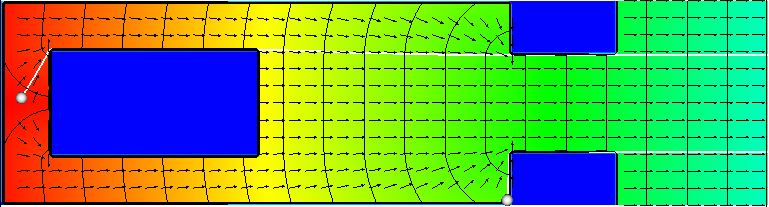
\includegraphics[width=0.9\linewidth]{pics/BottleneckObstaclePure}
\caption[Isolines of a floor-field.]{}
\label{fig:BottleneckObstaclePure}
\end{figure}

Given a discretization
of the domain \textgreek{W} and the target region ${\partial\Omega}$, the solution to the Eikonal Equation can be approached (angen�hert)
by using the Fast-Marching Algorithm. The algorithm provides a
first order approximation, yet sufficient for our cause (pedestrian
navigation). Computing-time of Fast-Marching is independent\footnote{Fast-Marching completion-time depends mainly on the length
 of the wavefronts. If the geometry leads to small lengths, as in geometries with large amounts of narrow corridors, completion
  time decreases.} of the complexity
of obstacles and walls. 

The negative gradient $-\nabla u$  of the ``first-arrival-times'' will 
be a useful tool in the routing of pedestrians/agents to the target region 
used as part of the algorithm's input. The Fast-Marching algorithm is 
described in the appendix in detail for further reference.

We will refer to the result of the Fast-Marching Algorithm as ``floor-field''.
To successfully use these floor-fields, we will discuss and analyze
a modification, which gives us a smooth floor-field, as proposed in roboticslab.uc3m.es.\label{replace with bibtex: http://roboticslab.uc3m.es/roboticslab/researchtopic/fast-marching}

\subsection{Safe Navigation using the Floorfield}

When using the plain approximation to the Eikonal Solution, agents
anticipate a non-smooth pathway that leads very close to 
walls (see white trajectories in figure \ref{fig:BottleneckObstaclePure}). 
In most of the models for pedestrian dynamics, pedestrians, which are very
close to walls or obstacles, could overlap with them in rare occasions.
Agents might leave the valid domain and find themselves captured inside
walls or obstacles. In the model described in this paper, we aim to fix that
problem. In reality, we can observe, pedestrians avoiding
walls and obstacles through keeping a certain distance. 

Therefore, it is desirable to define a modified quality of an optimal
route, which accounts for a minimal arrival time and a safe pathway.
Safe in respect to avoiding the vicinity of walls and obstacles, if
and only if possible. If a space is very crowded (high density), then 
agents should make use of the given space even if that means getting 
close to walls.

This crowd behavior, described above, is commonly achieved with adding 
a repulsive characteristic to walls.

In the ``social force model'', the walls
will have a repulsive force pointing perpendicular to the wall-surface, aiming to
keep agents away from the wall. These forces need to be calibrated
to work as intended.

Smaller forces might not be strong enough to avoid 
overlapping with the wall if an agent is in between a wall on one side 
and many other agents on the other side . The agents on the
other side affect that one agent, forcing him towards the wall,
while the wall itself acts on the agent in the opposite direction.

If the repulsive wall forces are too strong, pedestrians will not
use the space close to a wall, even if the domain is very crowded.

It is a difficult task, to find a set of parameters, that work as desired
in a broad set of situations and geometries.

Instead of modeling the repulsive character of walls (seen as
the avoidance of walls by pedestrians) via repulsive wall forces (social
force model), we modify the floor-field in a way, that pathways avoid
the vicinity of walls to a certain, adjustable degree, thus integrating
this repulsive character into the navigation/routing.

How can an agent ``avoid'' the close vicinity of any wall or obstacle?

\subsection{Distances-Field}

Having above question in mind, we first need to introduce and understand 
the \textit{Distances-Field}, a function $d$ living on the spacial domain $\Omega$, 
which holds information, how 
far away the closest wall is. This 
function will prove useful when altering the floor-field used for routing.

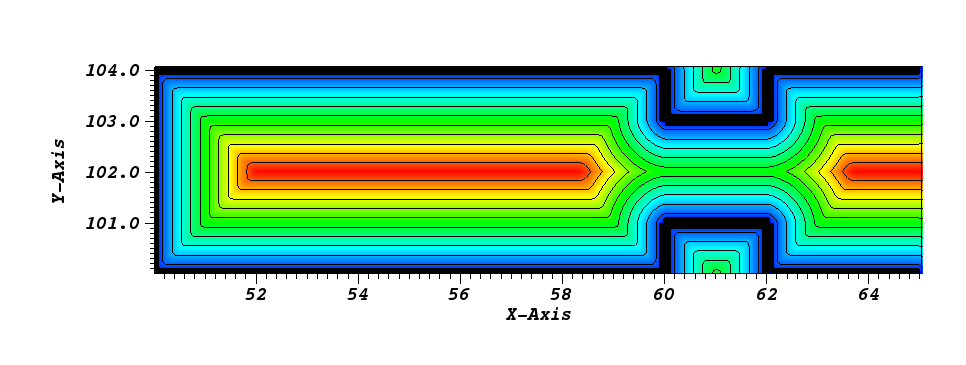
\includegraphics[width=0.9\linewidth]{pics/DistanceField2}
\label{fig:DistanceField2}

The function value $d(\vec{x})$ on the discrete grid, used for navigation, will
be used to create a slowness-map. This slowness-map will assign to each grid-point 
the value, which describes, how slow the 2-D wave will propagate over that grid-point.
Points, that are relatively close to a wall, will have a relatively low value $d(\vec{x})$.
Therefore, the 2-D wavefront will slow-down over these points. Routes passing these points
will take more time and be less optimal in a sense, that combines distances and wall-avoidance.


In the later, we will see two different floor-fields, which will have two 
different names, yet they are both created by using the 
Fast-Marching algorithm:
\begin{enumerate}
\item Direction-to-Wall-Field: this vector field holds the normalized direction to the closest wall
\item Navigation-Field: this vector field holds the negative gradient of the altered floorfield
\end{enumerate}

<< explain the pre-step incl. the threshold "cut-off"; have some nice pictures >>

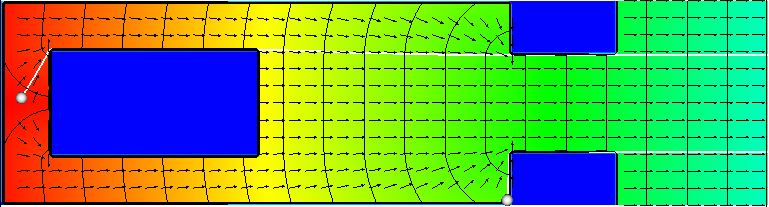
\includegraphics[width=0.8\linewidth]{pics/BottleneckObstaclePure}
%\caption[Isolines of a floor-field.]{}
\label{fig:BottleneckObstaclePure2}
the floor-field

$ \qquad \qquad \qquad \qquad \qquad \qquad \qquad \qquad \qquad \Downarrow $

$ \qquad \qquad $ is modified to:
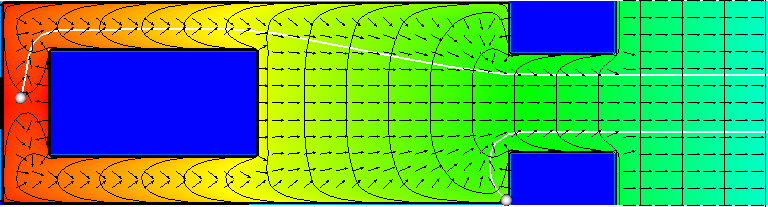
\includegraphics[width=0.8\linewidth]{pics/BottleneckObstacleEnhanced}
%\caption[Isolines of an enhanced floor-field.]{}
\label{fig:BottleneckObstacleEnhanced}




\subsubsection{Cost of a ``full'' preprocessing step }

<< the effort is doubled - but useful information is gained, that can be used in
more than one way. >>

Close to all time of the needed computation spent on the goal, the prohibition of overlapping, is
spent in a preprocessing step before the actual simulation starts and therefore does not
effect the real-time factor. A factor, which is a promintent metric, when comparing different models.

\subsubsection{Distances-Field and repulsive Wall-Forces}

<< optional? describe in short that the distance field takes responsibility for not
clipping in two ways: redirect in wall-distance < 0.2; modify floor-field to avoid walls >>

<< move this section >>

\subsection{Idea of Separation of a Moving-Vector into Direction and Magnitute}

\subsubsection{no clipping}

\subsubsection{Recycling the Distances Field (neg. Gradient must be saved)}

%$\vec{v}_{res}\quad=\quad\bigg(1-\frac{1}{2}\bigg[\langle\vec{v}_{n},(-\nabla distances)_{n}\rangle+\big\vert\langle\vec{v}_{n},(-\nabla distances)_{n}\rangle\big\vert\bigg]\bigg)\cdot\vec{v}_{n}$

\section{Testing}
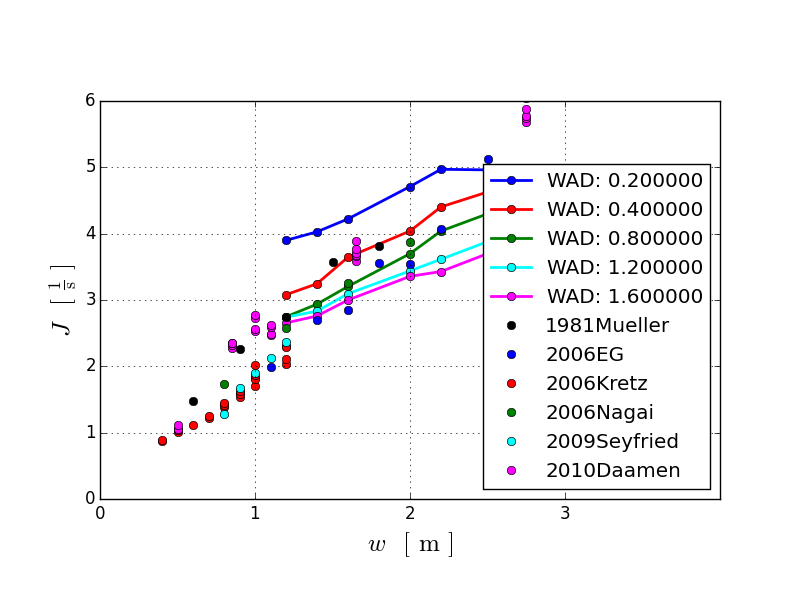
\includegraphics[width=0.9\textwidth]{pics/sim_flow_vs_experimental_data}
\section{Outlook}

\subsection{Floor-field}

\subsubsection{Multiple Goals }

The floor-field is a useful tool in routing of pedestrians through
any geometry. 

\subsubsection{Multiple Floors}

\paragraph{Neighboring Relations}

\subsection{Usage in JuPedSim}

\subsection{Floor-fields in Triangulated Domains}

\subsection{Parallelization}

\section{Appendices}

\subsection{Fast-Marching Algorithm}

\subsection{Classes and their Relations}

\subsection{Code Snippets}

\section{Bibliography}

\end{document}
